% !TEX root = QlockToo.tex

\begin{figure}
    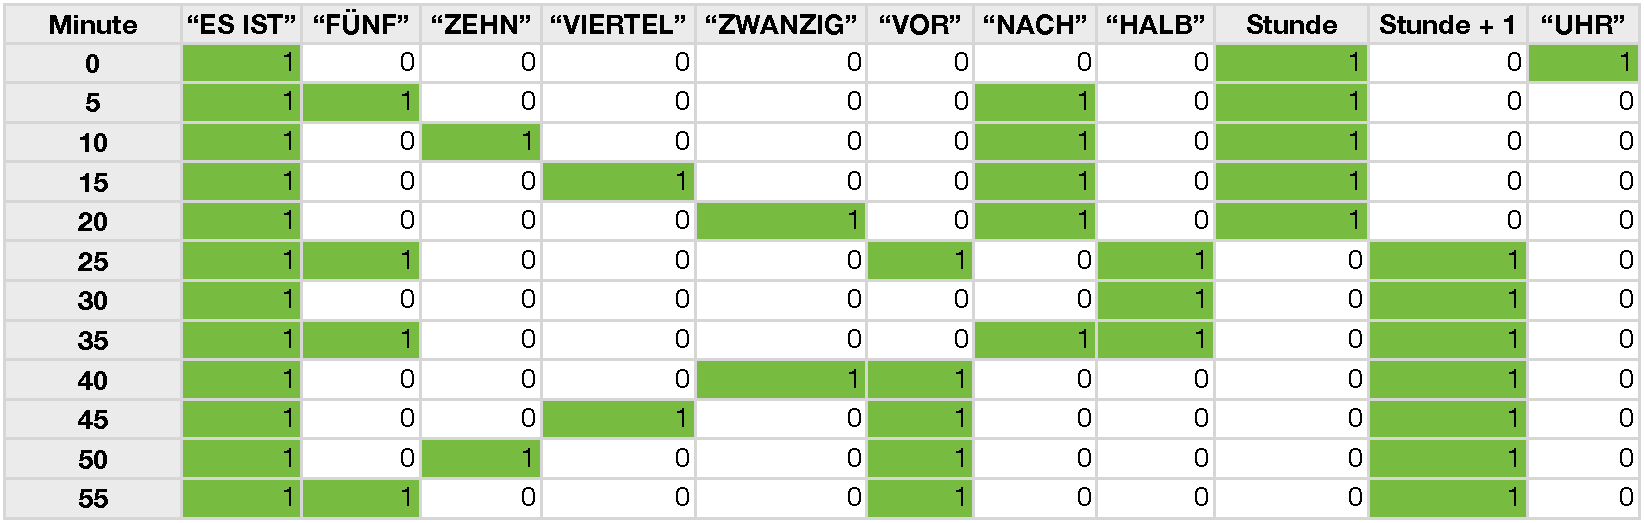
\includegraphics[width=\columnwidth]{Abbildungen/Firmware/Logik}
    \caption{Für die Anzeige der Zeit in Sätzen wird die dargestellte Logiktabelle für die deutsche Sprache in der Firmware hinterlegt. \emph{Stunde} und \emph{Stunde + 1} sind Platzhalter für die aktuelle und die nächste Stunde.}
    \label{fig:Logik}
\end{figure}

\section{Firmware}
\label{sec:Firmware}
Die Firmware der QlockToo ist in \emph{C} geschrieben und nutzt Funktionen des Arduino-Cores.
Im Folgenden werden die einzelnen Module der Firmware kurz erläutert.

\begin{multicols}{2}
\textbf{Firmware}
Die Hauptdatei der Firmware enthält den Einstiegspunkt in das Programm und initialisiert alle Module. Hier wird der Haupttimer (1kHz) gestartet, der Displayanzeige und Steuerungsfunktionen übernimmt.

\textbf{Display}
Im Display-Modul wird die Verbindung mit dem I2C-LED-Treiber hergestellt und die Ports für die Ansteuerung der Leistungstransistoren werden konfiguriert.

In der Display-Update-Routine findet das eigentliche Multiplexing statt. Es wird jeweils die nächste LED-Reihe eingeschaltet und die darzustellenden Spalten über die I2C-Schnittstelle an den LED-Treiber gesendet.
Diese Funktion ist besonders zeitkritisch, da ineffiziente Programmierung hier sofort zu einem flimmernden Bild führt.
Die QlockToo baut das Bild 100 mal pro Sekunde komplett auf (Multiplexing mit 1kHz über zehn Reihen), mit bloßen Auge ist daher kein Flimmern zu erkennen.

\textbf{Controller}
Im Controller-Modul befindet sich ein Zustandsautomat, welcher den Betriebsmodus (Zeitanzeige, Temperaturanzeige, usw.) verwaltet.
Der Betriebsmodus der Uhr kann über die Taster eingestellt werden. Das dazu notwendige Abfragen der Taster findet ebenfalls in diesem Modul statt.

\textbf{Timewords}
In diesem Modul ist die in Abbildung~\ref{fig:Logik} dargestellte Logiktabelle implementiert.
Welche LEDs für die gewählten Wörter und Stunden zu beleuchten sind, wird für jedes Wort in Form eines Integers für die Reihe und einer Bitmaske für die Spalten definiert.

\textbf{Api}
Die QlockToo kommuniziert per USB über das UART-Protokoll bei 115200 baud mit der Software.
Zum Parsen der empfangenen Befehle wird auf Seite der Firmware die Library \emph{SerialCommand}\footnote{https://github.com/kroimon/Arduino-SerialCommand} eingesetzt.

\textbf{Brightness}
Das Modul Brightness beinhaltet die Steuerung der Helligkeit der QlockToo. Neben dem Automatikmodus, welcher die Helligkeit der Abhängigkeit von den gemessenen Werten des Helligkeitssensors steuert, besteht die Möglichkeit einer manuellen Steuerung. Dabei stehen verschiedene Abstufungen zur Verfügung.

\textbf{DCF77}
In diesem Modul ist der Parser für das DCF77 Signal implementiert. Das DCF77-Signal ist zeitkritisch und wird daher in einem dedizierten Interrupt bearbeitet.
Sobald alle notwendigen Daten vorhanden sind -- was mindestens eine Minute dauert -- und der Paritätscheck erfolgreich ist, wird die globale interne Uhrzeit eingestellt.

\textbf{Matrix}
Im Modul \emph{Matrix} sind Funktionen zu Manipulation der Anzeigematrix zusammengefasst. Diese reichen vom Leeren und Füllen der Matrix hin zum Anzeigen von Zahlen und Buchstaben. Die Schriftarten sind in der Datei \emph{font.h} hinterlegt.

\textbf{Thermo}
Dieses Modul enthält die Umrechnung der gemessenen Spannung am Thermistor in eine Temperatur in Celsius.
Dazu kommen Anzeigefunktionen, die die Temperatur auf dem Display ausgeben.
Für die Anzeige der Temperatur wird eine kleinere Schriftart (3x5) genutzt als für die Anzeige der Sekunden (5x7), da noch das Gradzeichen angezeigt wird.

\textbf{Time}
Die QlockToo nutzt den internen 16-Bit Timer1 dazu, die Zeit einzuhalten.
Der Timer wird mit einem Prescaler von 256 Overflow-Betrieb genutzt und mit dem Wert 3036 vorgeladen.
Dadurch feuert der Timer exakt sekündlich und zählt Minuten und Stunden hoch.

\end{multicols}
